\documentclass{exam}

\input{preamble.sty}
\begin{document}
\begin{center}
    \Large
\textbf{Lab 9: Exploring VQE and Molecular Physics}
\end{center}
    \section{Potential Energy Curve of H$_2$}
    Using qiskit we are able to simulate the ground-state energy of H$_2$ for different bond lengths (8 lengths between 0.4\textup{~\AA} and 2.2\textup{~\AA}).
    To start off, the VQE was used to compute the groundstate energy. The n\_local algorithm was used to optimize the parameters and the initial ansatz was created using n\_local.
    The resulting energies with this set-up are shown below. 
    \begin{center}
        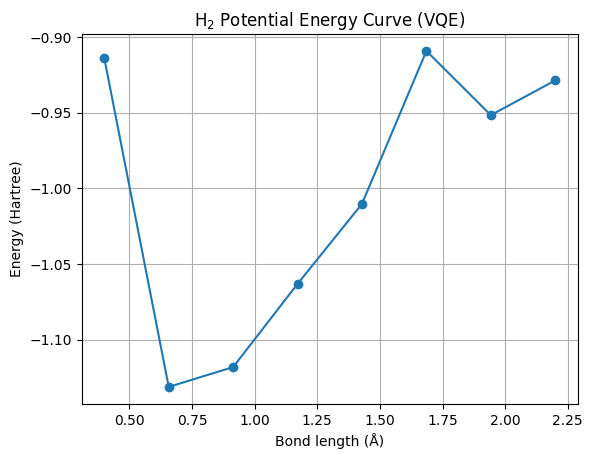
\includegraphics[width = .75 \linewidth]{images/graph1.png}
    \end{center}
    \section{Exploring Algorithmic Choices}
        \subsection{Changing the Ansatz}
            The same set-up is run again except this time the ansatz circuit, n\_local is replaced with EfficientSU2. 
            With the new ansatz, the resulting energies can be compared with the n\_local run.
            \begin{center}
                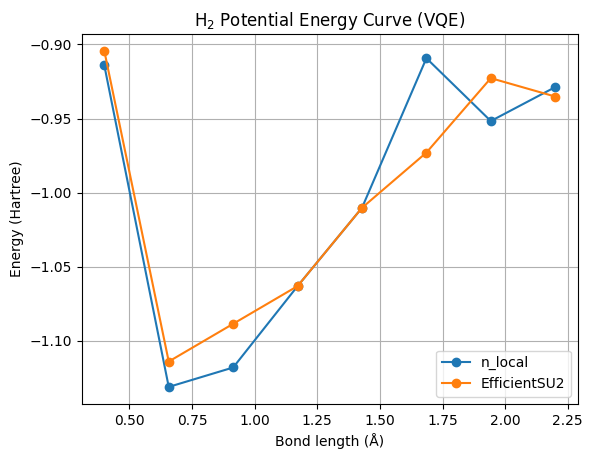
\includegraphics[width = .75 \linewidth]{images/graph2.png}
            \end{center}
            \subsubsection{Questions}
                \begin{itemize}
                    \item Does the energy decrease?
                    \begin{itemize}
                        \item The energy does approach 0 overtime, after an initial jump from .4\textup{~\AA} to .7\textup{~\AA}.
                    \end{itemize}
                    \item Is convergence faster or slower?
                    \begin{itemize}
                        \item Compared to the n\_local, the convergence rate is slower, but more stable. The graph as a much nicer curve when exluding the two endpoints.
                    \end{itemize}
                \end{itemize}
        \subsection{Changing the Optimizer}
            The same set-up is run for a third time, where we keep the EfficientSU2 circuit but replace the optimizer algorithm.
            Before the optimizer algorithm was SLSQP, now COBYLA will be used. Once again the results are compared with the two previous runs.
            \begin{center}
                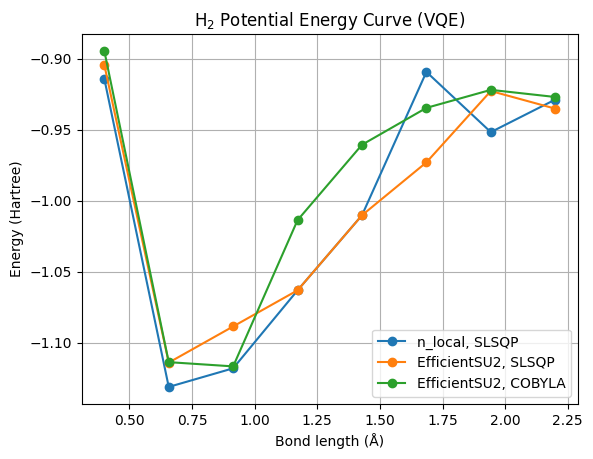
\includegraphics[width = .75 \linewidth]{images/graph3.png}
            \end{center}
            \subsubsection{Questions}
                \begin{itemize}
                    \item Is the optimization more stable?
                    \begin{itemize}
                        \item Yes, this optimization algorithm gives a very nice curve and has very small spikes compared to the other two curves. 
                    \end{itemize}
                    \item Does it reach the same minimum energy?
                    \begin{itemize}
                        \item Yes, all three have a final energy of around $.93 \pm +.01$. The n\_local run with the SLSQP algorithm does have a lower energy at a lower bond length and all three start off with a lower energy but they all end at around the same energy.
                    \end{itemize}
                \end{itemize}
    \section{Benchmarking and Interpretation}
        For the final run qiskits NumPuMinimumEigensolver is used to calculate the exact classical solution.
        \begin{center}
                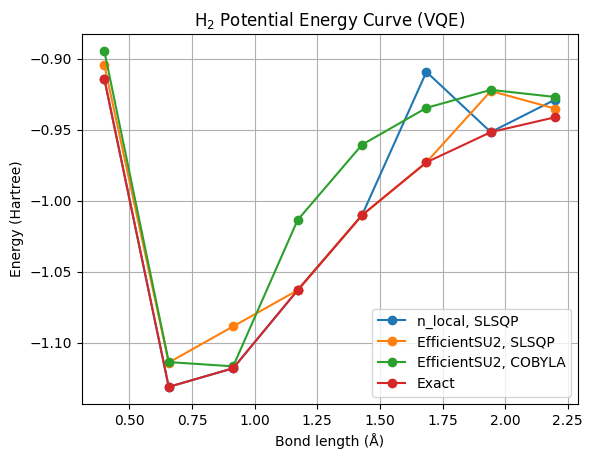
\includegraphics[width = .75 \linewidth]{images/graph4.png}
        \end{center}
            \subsubsection{Questions}
                \begin{itemize}
                    \item How close is VQE to the exact energy?
                    \begin{itemize}
                        \item Using VQE is relativily close to the exact energies, however each change gets different results. With n\_local and SLSQP the larger bond lengths seem to be the most accurate with the exact curve. With EfficientSU2 and SLSQP, the smaller bond lengths are closer. With EfficientSU2 and COBYLA, the energies are a bit higher that the exact but the shape of the curve matches alot better. 
                    \end{itemize}
                    \item Where do discrepencies come from?
                    \begin{itemize}
                        \item Discrepencies can arise from the optimization algorithm not being able to find the smallest energy and from the ansatz not being strong enough.
                    \end{itemize}
                \end{itemize}
    \section{Discussion and Wrap-Up}
        \begin{itemize}
            \item Which part of this lab was quantum?
            \begin{itemize}
                \item The estimator and ansatz are the quantum parts. The ansatz is a basline quess based off of a trial wavefunction and the quantum system. The estimator simulates a quantum computer to evaluate the Hamiltonian.
            \end{itemize}
            \item Which part was classical?
            \begin{itemize}
                \item The optimizer is the clasical part. It uses a classsical optimizer to find the best values for the given inputs, guiding the quantum circuit.
            \end{itemize}
            \item What currently limits the accuracy of VQE the most?
            \begin{itemize}
                \item Hardware noise from gate errors and decoherence along with shallow circuit depths.
            \end{itemize}
        \end{itemize} 
\end{document}